\UseRawInputEncoding
\documentclass[a4paper,12pt,twoside,openright]{book}
% Headers and macros defined
\usepackage[utf8]{inputenc}
%\usepackage[titletoc]{appendix}
\usepackage[toc,page]{appendix}
\usepackage{graphicx}
\usepackage{subfig}
\usepackage[spanish]{babel}
\usepackage{fancyhdr}
\usepackage{ae}
\usepackage[inner=3.0cm,outer=2.5cm,top=3cm,bottom=3cm]{geometry}
\usepackage[printonlyused]{acronym}
\usepackage{hlundef}
\usepackage{tesis}
\usepackage[inline]{enumitem}
\usepackage[usenames,dvipsnames,table,xcdraw]{xcolor}
\usepackage{dsfont}
\usepackage{algorithm}% http://ctan.org/pkg/algorithms
\usepackage{algpseudocode}% http://ctan.org/pkg/algorithmicx
\usepackage{amsmath, amsthm, amssymb, amsfonts}
\usepackage{breakcites}
\usepackage{xcolor}
\usepackage{color,soul}
\usepackage{multirow}
\usepackage{tikz,pgfplots,pgfplotstable}
\usepackage{capt-of}
\usepackage{csvsimple}
\usepackage{caption}
% change color of short text on acronyms
\AtBeginEnvironment{acronym}{
  \renewcommand*{\aclabelfont}[1]{\textbf{\acsfont{\color{blue}#1}}}
}
\usepackage{enumitem}
\usepackage[colorinlistoftodos]{todonotes}
\usepackage{mathrsfs}
\newtheorem{proposicion}{Proposición}[section]
\usepackage{amsfonts}
\usepackage{etoolbox}
\usepackage[group-separator={,}]{siunitx}
\usepackage{booktabs}
\newcommand{\ra}[1]{\renewcommand{\arraystretch}{#1}}
\setcounter{secnumdepth}{3}
\usepackage{filecontents,pgfplots,pgfplotstable}
\pgfplotsset{compat=1.13}
\usepgfplotslibrary{colormaps}
\usepackage{sidecap}
\usepackage{natbib}
% Define color for hyperref library used on content and acronyms
\definecolor{purple2}{rgb}{0.3, 0.12, 0.3} 
\usepackage[colorlinks=true]{hyperref}
\hypersetup{citecolor=blue}
\hypersetup{urlcolor=red}
\hypersetup{linkcolor=purple2}
\usepackage{cleveref}
\usepackage{tikz-qtree}
\usepackage{arydshln}
\usetikzlibrary{shapes.geometric, arrows, decorations.pathreplacing, shadows,trees, positioning, calc, tikzmark, spy, mindmap, matrix}
\tikzstyle{roundedFrame} = [rectangle, text centered, rounded corners, draw=gray]
\tikzstyle{input} = [rectangle,text centered, draw=none]
\tikzstyle{emptyFrame} = [rectangle,text centered, draw=white]
\tikzstyle{frame} = [rectangle, text centered, draw=gray]
\tikzstyle{arrow} = [thick,->,>=stealth]
\usepackage{pifont} % DING
\pagenumbering{Roman}
% line for define definitions
\newtheorem{defn}{Definition}[section]
% lines for translate appendix package to spanish
 \addto\captionsspanish{
     \renewcommand{\appendixtocname}{Apéndices}
     \renewcommand{\appendixpagename}{Apéndices}
 }
% define colors
\definecolor{pastelblue}{rgb}{0.68, 0.78, 0.81}
\definecolor{pastelorange}{rgb}{1.0, 0.7, 0.28}
\definecolor{pastelyellow}{rgb}{0.99, 0.99, 0.59}
\definecolor{pastelred}{rgb}{1.0, 0.41, 0.38}
\definecolor{pastelgreen}{rgb}{0.47, 0.87, 0.47}
\definecolor{error}{rgb}{1.0, 0.41, 0.38} % red
\definecolor{note}{rgb}{0.99, 0.99, 0.59} % yellow
\definecolor{info}{rgb}{0.68, 0.78, 0.81} % blue
\definecolor{tip}{rgb}{0.47, 0.87, 0.47} % green
\definecolor{Gray}{gray}{0.75}
\definecolor{LightCyan}{rgb}{0.88,1,1}

 
\title{Título de tesis}
\author{Nombre completo del autor de la tesis}
\orientador{Dr. / Magíster Nombre de Asesor}
\coorientador{Dr. / Magíster co-asesor (de ser el caso) }

\dedicado{ Aquí deberás colocar a quien va dedicada tu tesis por ejemplo, a todos los profesores por sus enseñanzas y algunos amigos}

\begin{document}
\maketitle 
%%%%%%%%%%%%%%%%%%%%%%%%%%%%%%%%%%%%%%%%%%%%%%%%%%%%%%%%%%%%%%%%%%%%
% Compone la carátula y la dedicatoria
%mayores detalles de como usas las abreviaturas (acronimos)
% vea: http://www.ctan.org/tex-archive/macros/latex/contrib/acronym/
% hay un manual en pdf en esa misma direccion

\chapter*{Acrónimos}

\begin{acronym}

\acro{AP}{Affinity Propagation}
\acro{CMM}{\emph{Capability Maturity Model}}
\acro{GPS} {Global Positioning System}
\acro{PCA}{Principal Component Analysis}
\acro{PLSIC}{Partial Least Squares Image Clustering}
\acro{RGB}{Red, Green, Blue}
\acro{SHNN-CAD}{Sequential Hausdorff Nearest-Neighbor Conformal Anomaly Detector}
\acro{SIFT}{Scale-Invariant Feature Transform}
\acro{t-SNE}{t-Distributed Stochastic Neighbor Embedding}
\acro{SPC}{Sociedad Peruana de Computación}

\end{acronym}

\begin{agradecimientos}
Aquí deberás colocar a quien y porque agradeces. Ejemplo:
En primer lugar deseo agradecer a Dios por haberme guiado.
Deseo agradecer de forma especial a mis docentes: nombre 1, nombre 2, nombre 3 porque fueron ejemplos que deseo seguir en mi vida profesional.
Deseo agradecer al personal administrativo de la universidad: nombre 1, nombre 2, nombre 3. Muchas gracias por la atención brindada y porque siempre estuvieron dispuestas a ayudarnos.
\end{agradecimientos}
 %Inserta los agradecimientos
\begin{resumen}

% Insertando imagen.
  \begin{figure}[!htb]
  \centering
  \subfloat{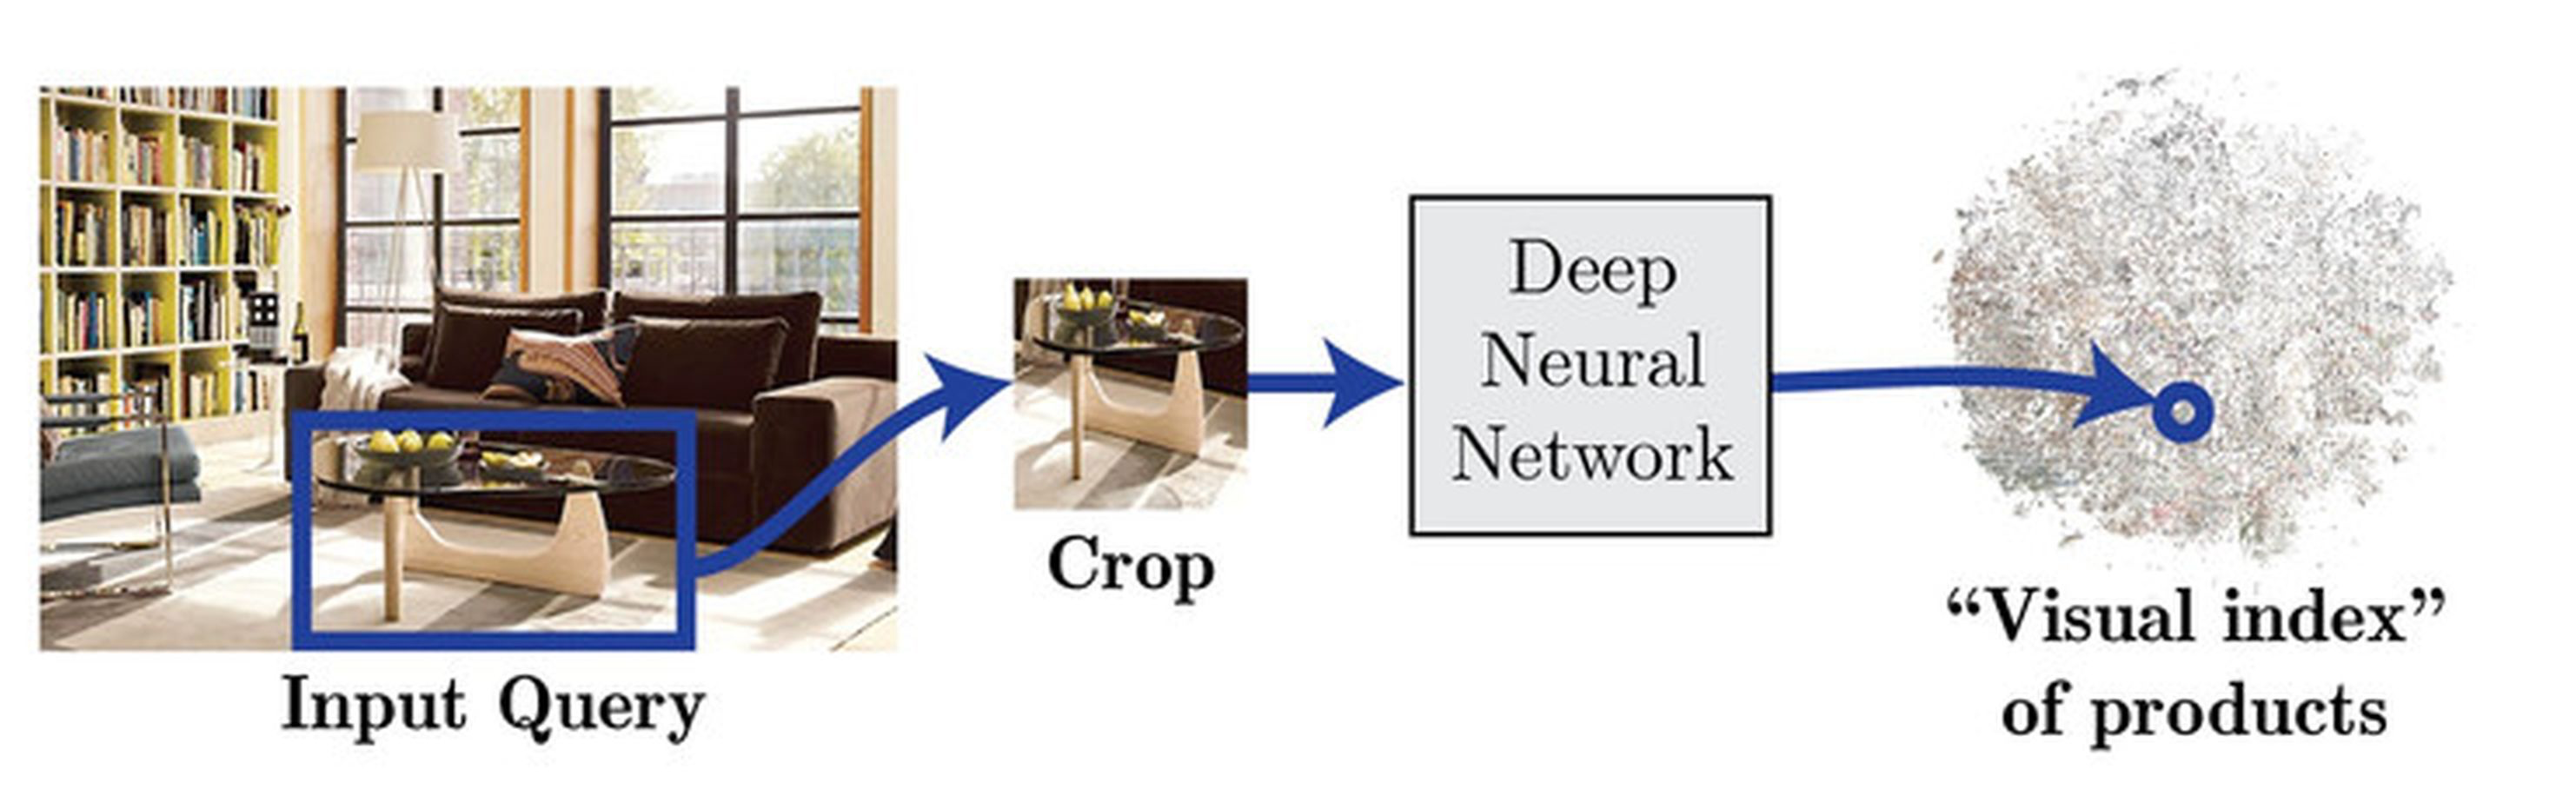
\includegraphics[width=5.7in]{graficos/Abstract}}
  \label{fig:Attrib2}
  \end{figure}
% Fin de figura MOdificado

Aquí deberas colocar entre 100 y 150 palabras como máximo, el problema que intentas resolver, la justificación y los aportes o soluciones que planteas.

\begin{flushleft}
\textbf{Palabras clave:} Inteligencia artificial, Programación paralela, Procesamiento de videos.
\end{flushleft}

\end{resumen}
 %Inserta el resumen
\begin{abstract}

Here you must write between 100 and 150 words about your thesis. 
In this text you must highlight your main contributions to this field.

\begin{flushleft}
\textbf{Keywords:} Intelligent systems, Parallel programming, Video processing.
\end{flushleft}

\end{abstract}
 %Inserta el abstract

%%%%%%%%%%%%%%%%%%%%%%%%% list of content %%%%%%%%%%%%%%%%%%%%%%%%
\tableofcontents %Inserta el índice general
\listoftables %Inserta el índice de cuadros
\addcontentsline{toc}{chapter}{Lista de Tablas}
\listoffigures %Inserta el índice de figuras
\addcontentsline{toc}{chapter}{Lista de Figuras}
%
%%%%%%%%%%%%%%%%%%%%%%%%%%%%%%%%%%%%%%%%%%%%%%%%%%%%%%%%%%%%%%%%%%
%%%   En esta parte deberas incluir los archivos de tu tesis   %%%
%%%%%%%%%%%%%%%%%%%%%%%%%%%%%%%%%%%%%%%%%%%%%%%%%%%%%%%%%%%%%%%%%%
%
\clearpage 
\pagenumbering{arabic}
\chapter{Introducción}
\label{chap:cha1}

Este es el primer capítulo de la tesis. Se inicia con el desarrollo de la introducción de la tesis. En esta parte debes explicar que es lo que se presenta en el trabajo. ¿Por que se escogio este método?. Es importante que el texto utilice la tabla de abreviaturas correctamente. En el archivo abreviaturas.tex contiene la tabla de abreviaturas. Para citar alguna de ellas debes usar los comandos $\backslash$ac\{tu-sigla-aqui\}. Si es la primera vez que utilizas la sigla ella se expandirá por completo. Por ejemplo, el comando $\backslash$ac\{CMM\} va a producir: \ac{CMM}. Si más adelante repites el mismo comando sólo aparecerá la sigla \ac{CMM}. Para explorar mucho más este comando es necesario leer su manual disponible en: \href{http://www.ctan.org/tex-archive/macros/latex/contrib/acronym/}{Link referencia}.


\textbf{Hipótesis}.
Nuestra hipótesis consiste de la siguiente proposición: \textit{ Texto de la hipótesis}.


\section{El problema}
(En esta sección se realiza el planteamiento del problema que queremos resolver con la tesis. Sea muy puntual y no ocupe más de un párrafo en especificar cual es el problema que desea atacar)


\section{Justificación y motivación}
(En esta sección se va desde aspectos generales a aspectos específicos (como un embudo). No se olvide que es la primera parte que tiene contacto con el lector y que hará que este se interese en el tema a investigar).



\textbf{Justificación}.
A quien beneficia el trabajo de investigación una vez culminado, como se beneficia. y.
Especificar el problema que se va enfrentar 

\textbf{Motivación}.
¿Por qué es importante?, mensionar el aporte.


\section{Objectivo General}
En esta sección se colocan los objetivos generales de la tesis. Máximo dos. Si necesita ampliar estos objetivos utilice la sección de objetivos específicos.


\subsection{Objetivos Específicos}
En esta sección los objetivos especificos de la tesis son mencionados las cuales responderan las preguntas de la investigación.
 \begin{enumerate}
 	
	\item Primer objetivo.
	
	\item Segundo objetivo.
	
 	\item Tercer objetivo.
	
 \end{enumerate}

%\section{Contributions}

\section{Organización del texto}
Aquí deberas colocar como esta organizado tu texto.

\chapter{Marco Teórico}
\label{chap:cha2}

Cada capítulo deberá contener una breve introducción que describe en forma rápida el contenido del mismo. En este capítulo va el marco teórico. (pueden ser dos capítulos de marco teórico)

Este capítulo presenta conceptos relacionados a nuestro método o abordaje de modo que el lector pueda familiarizarse con los temas expuestos.


Ejemplo de como escribir seudo código en latex.
\begin{algorithm}[!htb]
	\caption{\ac{AP}.}\label{alg:ap}
	\begin{algorithmic}[1]
		\Procedure{ClusteringAP}{$S$}
		\State $R(i,k) = 0, ~A(i,j)= 0, ~ \forall i,k$
		
		\While{ Until converge }
		\State $R(i,k) = S(i,k) - max(A(i,j) + S(i,j))~|~ (j \in [1,n]; j\neq k) $
		
		\State $A(i,k) = min (0, R(k,k) + \sum_j max(0, R(j,k))), ~|~ (j \in [1,n]; ~j\neq i; ~j\neq k )$
		
		\State $A(k,k) = \sum_i max(0,R(i,k)) , ~|~ (i \neq k)$ 
		
		\EndWhile
		\State \textbf{return} $Trks$
		\EndProcedure
	\end{algorithmic}
\end{algorithm} 

Ejemplo de como hacer definiciones en latex:

\begin{defn}
Given a set of $n + 1$ data points $(x_i, y_i)$ where no two $x_i$ are the same, there is a polynomial $p$ of degree at most $n$ with the property $p(x_i) = y_i$, $i=0,\ldots,n$.
\end{defn}

Ejemplo de ecuaciones: 
\begin{equation}
	\label{eqn:interpolation}
	 p(x) = a_n x^n + a_{n-1} x^{n-1} + \cdots + a_2 x^2 + a_1 x + a_0
\end{equation}

%\subsubsection{Sub sub sección} 
 
 Ejemplo de utilización de abreviaturas, \ac{SPC}.
 
 
\chapter{Trabajos Relacionados}
\label{chap:cha3}

En este capítulo está destinado a explicar el estado del arte de las investigaciones relacionadas a la propuesta de tesis.
Este capítulo debe contener un buen número de referencias y no debe exceder tres páginas de texto. Para esto se puede tomar como ejemplo la forma de hacer una revisión bibliográfica en un artículo científico.

Este es un ejemplo de como realizar una referencia implícita \citep{Yasmin2015} y unas referencias explícitas \citet{Furini2008, Avila2011}.


La figura \ref{fig:Pipeline2} es un ejemplo de como insertar y referenciar una imagen.
Este es un ejemplo de enumerado.


\begin{enumerate*}
\item[(a)] Primer item
\item[(b)] Segundo item
\item[(c)] Tercer item
\end{enumerate*}.


Ejemplo de como insertar imagenes:
% Insertando imagen.
  \begin{figure}
  \centering
  \subfloat[]{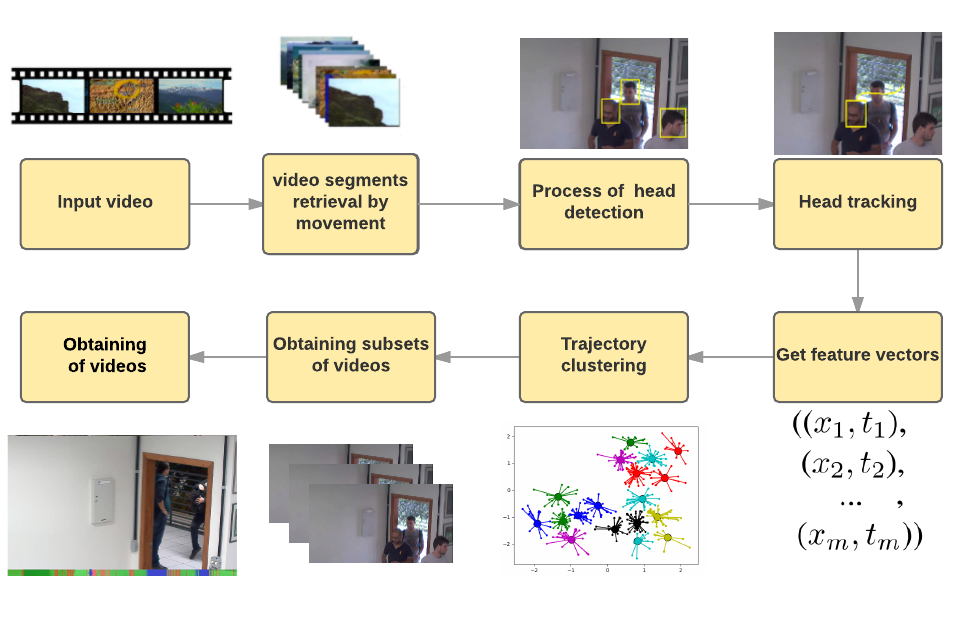
\includegraphics[width=6in]{graficos/pipeline2.png}}
  \caption[Imagen ilustrativa.]
  {Imagen ilustrativa. Imagen ilustrativa de como se puede insertar una imagen con latex.}
  \label{fig:Pipeline2}
  \end{figure}
% Fin de insertando de imagen







\chapter{Metodología}
\label{chap:cha4}

(En este capítulo se desarrolla toda la propuesta realizada a través de la investigación. Sigue la misma estructura del capítulo anterior. El título del capítulo es flexible de acuerdo a cada tesis. Aqui va una introduccion para el pipeline).

\section{Método}
Este capítulo explica el enfoque o solución para el problema.


\section{Abordaje}
En este capítulo puedes explicar detalladamente en que consiste tu solución.

Aqui podemos observar un ejemplo para escribir una definición:

\begin{defn}
Un punto $p$ es una tupla $(x, y, t)$, donde $x$ y $y$ son las posiciones en la imagen y $t$ es el lapso de tiempo cuando el punto es colectado, donde $k$ $\in$ $\mathds{N}$.
\begin{equation}
	p_k = (x_k,y_k,t_k).
\end{equation}
\end{defn}

%\noindent

Example of ecuación:
La ecuación \ref{equa:example}, es un ejemplo de como utilizar una ecuación.
\begin{equation}
    \label{equa:example}
	f(x_k) = y_k, k=1, ..., n
\end{equation}

\chapter{Pruebas y resultados}
\label{chap:cha5}
En este capítulo se comentan las pruebas hechas que validan el estudio, finalmente se comentan los resultados y conclusiones de esta tesis, así 

\section{Pruebas}

\section{Resultados}


La tabla \ref{table:example} es un ejemplo de como colocar tablas en latex.

% introducir la tabla conteo.
\begin{table}[h]
\centering
\scalebox{0.57}{
    	\begin{tabular}{cccccccc}
    	\hline
    	& Clustering & Clustering  \\
    	& SOM (\%) & Affinity (\%)  \\
    	\hline
    	\rowcolor{LightCyan}
    	Interpolation Descriptor & 22.28 & 15.67  \\
    	Fourier Descriptor & 9.90 & 9.20  \\
    	\rowcolor{LightCyan}
    	Wavelet Descriptor & 8.77 & \textbf{6.77}  \\	
    	\hline
    	\end{tabular}
	}
	\caption[Resultados con método propuesto.]{Porcentage de error obtenido.}
	\label{table:example}
\end{table}


\chapter{Conclusiones y Trabajos Futuros}\label{chap:conclusions}

Las conclusiones de la tesis son una parte muy importante y tiene las siguientes partes.

En primer lugar debes escribir las conclusiones generales de tu trabajo, evita escribir en forma de viñetas. Simplemente utiliza texto continuo. En las concluciones es posible mencionar que es lo que se aprendio en el estudio de manera resumida. Realizar una conclucion no tienes que detallar como fue visto en los experimentos, las conclusiones son mejor apreciadas si son profundas.

\section{Limitaciones}
La segunda  parte de este capítulo corresponde a las limitaciones que tiene la propuesta. Esta seccion es muy importante para que los siguientes estudiantes que hagan algo en esta línea no cometan los mismos errores y tu tesis sea un buen peldaño para avanzar más rápido.

\section{Recomendaciones}
En esta sección el tesista debe reflejar que la tesis ha permitido adquirir nuevos conocimientos que podrían servir para guiar otros trabajos en el futuro.

\section{Trabajos futuros}
En base a los puntos anteriores es recomendable que tu tesis también sugiera trabajos futuros. Esta sección es esencialmente útil para otras ideas de tesis. Todo este capítulo no debe ser más de cuatro páginas.


\begin{appendices}
\chapter{Título de Apéndice}
\section{Primer subtitulo}

  Insertando una imagen de prueba:
  %% insertar imagen
  \begin{figure}
  \centering
  \subfloat[]{\includegraphics[width=5in]{graficos/pipeline.pdf}}
  \caption[Figura en apéndice.]
  {Ilustraci\'on A.1: Esta es una figura de prueba para el apéndice.}
  \label{RoboAcci}
  \end{figure}

% Instrucción para no insertar la imagen en blanco
\let\cleardoublepage\clearpage
  
\chapter{Título Segundo Apéndice}
\section{Segundo subtitulo}
Aquí va el contenido del segundo Apéndice.

\end{appendices} % Insertando Apéndice

%%%%%%%%%%%%%%%%%%%%%%%%%%%%%%%%%%%%%%%%%%%%%%%%%%%%%%%%%%%%%%%%%
\bibliographystyle{authordate1}
\bibliography{contenido/bibliog}
\addcontentsline{toc}{chapter}{Bibliografía}
\end{document}
